% com-cas-poster
% by hk, rj, June 2012

\documentclass[final]{beamer} 

\mode<presentation> {  
    %\usetheme{Warsaw}
    \usetheme{Boadilla}
    %\usetheme{Montpellier}
    %\usetheme{Singapore}
    %\usetheme{Ilmenau}
    %\usetheme{Berkeley}
    %\usetheme{Madrid}
}

\usepackage[english]{babel}
%hk% \usepackage[latin1]{inputenc}
\usepackage{relsize}
\usepackage{listings}

\usepackage{epsfig}

\usepackage{amssymb}
%\usepackage{amsmath,amsthm, amssymb, latexsym}
\usefonttheme[onlymath]{serif}
\boldmath

\usepackage[orientation=landscape,size=a1,scale=1.4]{beamerposter}

\newcommand{\code}[1]{\texttt{#1}}


\title[Categories and Mixins]{Categories as classes and mixin composition}

\author[Kredel \& Jolly]{Heinz Kredel\inst{1} and Raphael Jolly\inst{2}} 

\institute{IT-Center, University of Mannheim, Germany %,
%\email{kredel@rz.uni-mannheim.de,}
\and Databeans, Paris, France%,
%\email{raphael.jolly@free.fr}
}

\date{CASC2012, September, 3-6, 2012}

\begin{document}

  %hk: makes new page% \maketitle

\begin{frame}[fragile] 
\frametitle{\mbox{ }\\ \hspace{13cm}Categories as classes and mixin composition, Heinz Kredel and Raphael Jolly}
%\hfill
\begin{columns}[t]

\begin{column}{.3\linewidth}

  \begin{block}{\large Contents}
  \normalsize 
  \begin{enumerate}
  \item generic, strongly typed, object oriented computer algebra software
  %\item concept of categories 
  \item software, algorithm implementations can be packaged and
    re-combined using traits in a category-like fashion
  \end{enumerate}
\tiny
{\scriptsize \textbf{Acknowledgments:}}
Thomas Becker, Wolfgang K. Seiler, Thomas Sturm, Axel Kramer, 
Jaime Gutierrez, Sherm Ostrowsky, Markus Aleksy
  \end{block}
  \hfill
  \begin{block}{\large Introduction}
\scriptsize
The modeling of algebraic structures in a strongly typed, generic,
object oriented computer algebra software has been presented with the
systems JAS \cite{Kredel:2000,Kredel:2008} and ScAS \cite{Jolly:2010}.
The design and implementation of these strongly typed, generic and
object oriented polynomial algorithm libraries in Java and Scala is
presented in \cite{JollyKredel:2010}. %,JollyKredel:2011}.
The libraries are enhanced for interactive usage with the help of the Jython and
JRuby scripting languages. The libraries now
provide several algorithm versions for greatest common divisor,
squarefree decomposition, factorization and Gr\"obner bases
computation in separate packages.

In this poster we discuss the problem of code organization and
algebraic structure configuration and deployment. Elements of algebraic
structures are implemented by classes and instantiated as objects with
methods implementing the `inner' algorithms of the structure in the
programming language. The algorithm libraries, for example the
construction of Gr\"obner bases, are kept in separate source code trees
and packages. This code organization helps in the separation of the
various possibilities for algorithm implementation and helps in the
transparent selection of appropriate algorithms for a given problem.
However, it is not always clear where to draw the line between `inner'
structure algorithms and `external' library algorithms.
  \end{block}
  \hfill
  \begin{block}{\large Generic, strongly typed, object oriented computer algebra software}
      \centering
      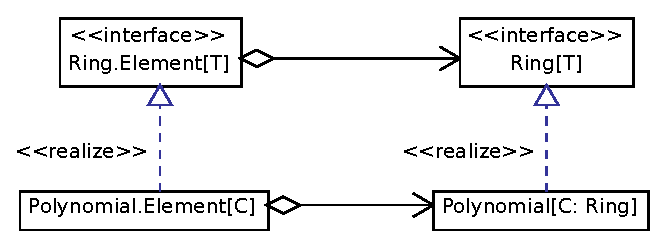
\epsfig{file=BasicTypes,clip=,width=0.85\linewidth}
  \end{block}
  \hfill
  \begin{block}{\large Example}
\tiny 
%code example in ScAS syntax - maybe we need to translate
%the uml diagram as well ?
\begin{lstlisting} 
 import scas._
 import Implicits.QQ
 implicit val r: Polynomial[Rational] = Polynomial.factory(QQ, "w")
 val Array(w) = r.generators
 val a: Polynomial.Element[Rational] = pow(w, 2) - 2 
\end{lstlisting} 
%
% val a = w**2 - 2 is this possible ?
% can we show the type of r, w and a ?
%
%\begin{verbatim} 
%BigRational rf = new BigRational(1); 
%GenPolynomialRing<BigRational> pf 
% = new GenPolynomialRing<BigRational>(rf,new String[]{"w"});
%GenPolynomial<BigRational> a = pf.parse("w^2 - 2");
%\end{verbatim}
  \end{block}
\end{column}


\begin{column}{.3\linewidth}
 
  \begin{block}{\large Algorithm libraries}
  \scriptsize 
  \begin{itemize}
  \item focus on multivariate polynomials over UFDs
  \item \textbf{greatest common divisor:} 
        interface \code{Greatest\-Common\-Divisor} with \code{gcd()}, \code{content()}, 
        implementations for various polynomial remainder sequence (PRS) algorithms: 
        simple, monic, primitive and the sub-resultant algorithm 
        generic for any (UFD) coefficient ring,
        other implementations use Chinese remainder algorithms or Hensel lifting
  \item \textbf{squarefree decomposition:} 
        interface \code{Square\-free}, 
        generic implementations for finite or infinite coefficient fields 
        or rings of characteristic $0$ or $p$
  \item \textbf{factorization:} 
        interface \code{Factorization}, 
        implementation depends on the explicit coefficient ring 
        but is generic in the sense that it can factor
        over arbitrary stacked coefficient field extensions, like mixed
        transcendental and algebraic extensions
  \item \textbf{factories} select appropriate algorithms for given coefficients
        %\code{GCD\-Factory}, \code{Squarefree\-Factory} and two \code{Factor\-Factory} classes. 
        %with methods \code{get\-Implemen\-tation(cofac)}
  \end{itemize}
  \end{block}
  \hfill
  \begin{block}{\large Code organization problem}
  \scriptsize
The algebraic structures and elements together with the algorithm
libraries provide a way to define precisely suitable combinations
for given situations. Depending on algorithm variations however,
the number of such combinations can become quickly huge and makes
some structuring principle be welcome.
%It is, however, elaborate and one would like to combine or
%package together certain configurations to be able to
%deploy and use them as a single object or thing.
  \end{block}
  \hfill
  \begin{block}{\large Categories in computer algebra systems}
  \scriptsize
  \begin{enumerate}
  \item Axiom, Aldor: abstract classes in OOP
        \cite{JenksSutor:1992, Watt:2003}
  \item Magma, Sage: classes with same representation
        \cite{BosmaCannonPlayoust:1997, Stein:2005}
  \end{enumerate}
  \end{block}
  \hfill
  \begin{block}{\large Mixins for category-like code organization}
\scriptsize
Reusable components \cite{Odersky:2005} consist in splitting software in
as many pieces as needed or possible, and to re-assemble these according
to the principle of composition. Hierarchical composition and peer
composition (also called mixin composition) are two variations of this
principle. We illustrate their respective usage with the example of GCD
computation. We consider components for each algorithm flavor and combine
them using either hierarchical or mixin composition. The code samples are
given in the computer language Scala using its concept of
{\em traits}.
  \end{block}
\hfill
  \begin{block}{\large References}
  \tiny %\scriptsize
  \bibliographystyle{abbrv}%{splncs}
  %\bibliography{com-cas-poster}
  %\def\newblock{}
\begin{thebibliography}{1}

\bibitem{BosmaCannonPlayoust:1997}
\def\newblock{}
W.~Bosma, J.~J. Cannon, and C.~Playoust.
\newblock The {Magma} algebra system {I}: The user language.
\newblock {\em J. Symb. Comput.}, 24(3/4):235--265, 1997.

\bibitem{JenksSutor:1992}
\def\newblock{}
R.~Jenks and R.~Sutor, editors.
\newblock {\em {axiom} The Scientific Computation System}.
\newblock Springer, 1992.

\bibitem{Jolly:2010}
\def\newblock{}
R.~Jolly.
\newblock {ScAS} - {Scala} algebra system.
\newblock Technical report, \\ https://github.com/rjolly/scas, accessed Jan
  2012, since 2010.

\bibitem{JollyKredel:2010}
\def\newblock{}
R.~Jolly and H.~Kredel.
\newblock Generic, type-safe and object oriented computer algebra software.
\newblock In {\em Proc. CASC 2010}, pages 162--177. Springer, LNCS 6244, 2010.

\bibitem{Kredel:2000}
\def\newblock{}
H.~Kredel.
\newblock The {Java} algebra system ({JAS}).
\newblock Technical report, http://krum.\-rz.uni-mann\-he\-im.de/jas/, accessed Jan
  2012, since 2000.

\bibitem{Kredel:2008}
\def\newblock{}
H.~Kredel.
\newblock On a {Java} {Computer} {Algebra} {System}, its performance and
  applications.
\newblock {\em Science of Computer Programming}, 70(2-3):185--207, 2008.

\bibitem{Odersky:2005}
\def\newblock{}
M.~Odersky and M.~Zenger.
\newblock Scalable component abstractions.
\newblock In {\em Proc. OOPSLA '05}, pages 41--57. ACM, 2005.

\bibitem{Stein:2005}
\def\newblock{}
W.~Stein.
\newblock {\em {SAGE} {M}athematics {S}oftware}.
\newblock The SAGE~Group, since 2005.
\newblock http://www.sagemath.org, accessed Oct 2011.

\bibitem{Watt:2003}
\def\newblock{}
S.~Watt.
\newblock Aldor.
\newblock In {\em Computer Algebra Handbook, Springer}, pages 265--270, 2003.

\end{thebibliography}

  \end{block}
\end{column}


\begin{column}{.3\linewidth}

  \begin{block}{\large Preliminary settings}
\tiny
\begin{lstlisting}
 import scas.structure.Ring // declares method plus etc.
 import Polynomial.Element
 trait Polynomial[C: Ring] extends Ring[Element[C]] {
   def plus(x: Element[C], y: Element[C]) = ...
   ...
 }
 object Polynomial {
   trait Element[C] extends Ring.Element[Element[C]]
 }
\end{lstlisting}
  \end{block}
  \hfill
  \begin{block}{\large Peer vs hierarchical composition}
\tiny
{\footnotesize In hierarchical composition, work is delegated to
a member ring:}
\begin{lstlisting}
 trait GCDEngine[C: Ring] {
   val ring: Polynomial[C]
   def gcd(x: Element[C], y: Element[C]): Element[C]
 }
 trait GCDSimple[C: Ring] extends GCDEngine[C] {
   def gcd(x: Element[C], y: Element[C]) = // use ring.plus etc.
 }
 val e = new GCDSimple[BigInteger] {
   val ring = new Polynomial[BigInteger]
 }
\end{lstlisting}
{\footnotesize The same effect can be obtained through inheritance
(peer composition):}
\begin{lstlisting}
 trait GCDSimple[C: Ring] extends Polynomial[C] {
   def gcd(x: Element[C], y: Element[C]) = // use this.plus etc.
 }
 val r = new GCDSimple[BigInteger]
\end{lstlisting}
{\footnotesize Delegation decouples components - inheritance increases coupling.}
  \end{block}
  \hfill
  \begin{block}{\large Mixin composition and categories}
\tiny
{\footnotesize In the mixin case, we can combine several
algorithms through multiple inheritance:}
\begin{lstlisting}
 trait GCDEngineX[C: Ring] extends Polynomial[C] {
   def gcd(x: Element[C], y: Element[C]) = ...
 }
 trait SquarefreeEngineY[C: Ring] extends Polynomial[C] {
   def squarefreePart(x: Element[C]): Element[C] = ...
   def squarefreeFactors(x: Element[C]): List[Element[C]] = ...
 }
 trait FactorEngineZ[C: Ring] extends Polynomial[C] {
   def factorList(x: Element[C]): List[Element[C]] = ...
   def factors(x: Element[C]): Map[Element[C], Long] = ...
 }
 val r = new GcdEngineX[BigRational] 
         with SquarefreeEngineY[BigRational]
         with FactorEngineZ[BigRational]
\end{lstlisting}
{\footnotesize Then \code{r} represents a polynomial category.
Some algorithms may need further specialization of the coefficient
type:}
\begin{lstlisting}
 trait GCDModular extends Polynomial[BigInteger] {
   def gcd(x: Element[BigInteger], y: Element[BigInteger]) = ...
 }
 val r = new GCDModular
\end{lstlisting}
{\footnotesize The desired packaging can be pre-setup or chosen
automatically according to the coefficient type:}
\begin{lstlisting}
 val r = Polynomial.factory(ring, pp)
\end{lstlisting}
{\footnotesize The \code{factory} method might return an object of type
\code{GCDModular} if ring is \code{BigInteger} and so on.
This category scheme using mixins ties together algebraic structures
with some specific algorithm implementations and so solves the packaging
problem.}
  \end{block}
\end{column}

\end{columns}

%\vfill
\end{frame}


%\begin{frame}[fragile] 
%\frametitle{Next page}
%\vfill
%\begin{columns}[t]
%\begin{column}{.3\linewidth}
%  \hfill
%\end{column}
%
%\begin{column}{.3\linewidth}
%  \begin{block}{\large Discussion}
%\scriptsize
%Mixin composition is interesting when there is a bidirectional dependency
%between two components. For instance in our example, the GCD algorithm
%needs a Polynomial ring, and the Polynomial ring needs a GCD algorithm,
%because its signature declares a gcd method. In all other cases,
%hierarchical composition may fulfill the need. There is a question
%whether e.g. factors or squarefreePart methods must be included in the
%signature of a UniqueFactorizationDomain, in which case mixin composition
%would be prefered.
%  \end{block}
%\end{column}
%
%\end{columns}
%
%\vfill
%\end{frame}

\end{document}
